\documentclass[12pt]{article}
	\usepackage{mgates-letter}
	\definecolor{dark_blue} {rgb}{0., 0., 0.65}
	
	\usepackage{textcomp}
	\usepackage{mathrsfs}  % mathscr font
	\usepackage{boxedminipage}
	\usepackage{rotating}
	\usepackage{svg}
	%\usepackage{natbib}
	\usepackage[colorlinks, filecolor=dark_blue, urlcolor=dark_blue, linkcolor=black, citecolor=black]{hyperref}
\begin{document}

\title{Towards AI-powered Swarm Engineering}
\author{Leonardo Micelli}
\date{\today}
\maketitle

\noindent


% ----------------------------------------
\setcounter{tocdepth}{2}

% set these after the TOC
\setlength{\parindent}{0em}
\setlength{\parskip}{1em}

% ----------------------------------------
\section{State of the Art}
\paragraph{\textbf{Collective Adaptive Systems and Macroprogramming}} Collective Adaptive Systems~\cite{ferscha2015collective} are large scale distributed systems composed of multiple autonomous, 
interacting entities that operate in open-ended environments. While each entity within the CAS (i.e., sensor, robot, software agent) operates autonomously with its own local context and objective, their interactions
produce \textbf{emergent global behaviors}. Decision-making in CAS is decentralized, and global functionality emerges from local interaction. Examples of CAS can be found in \textit{Smart Cities}, \textit{WSNs}, \textit{Digital Twins} and \textit{Swarm Robotics}.
CAS are typically heterogeneous and highly dynamic: entities can fail, join and leave at any time, introducing key challenges ranging from scalability and resource constraints to resilience and adaptability in
unpredictable environments. Novel approaches to the engineering of CAS propose to shift the focus from the individual entity to the collective as a whole \textit{(macroprogramming~\cite{10.1145/3579353})}, to manage increasing complexity while
improving maintainability. The main idea is to capture the macroscopic behavior of a collective system through a single program, abstracting away the complexities of individual components.

\paragraph{\textbf{Swarm Robotics}} Swarm robotics is an approach to collective robotics that draws inspiration from the self-organized behavior of social animals ~\cite{brambilla2013swarm}. The goal is to design robust, flexible and scalable 
collective behaviors for large number of robots through simple rules and local interactions. There are two main methods for designing such systems: \textit{automatic design}, which employs methods derived from
evolutionary robotics and multi-robot reinforcement learning, and \textit{behavior-based design}, which involves the design and implementation of algorithms that can be executed by the robots. This design approach is often realized
in a bottom-up fashion, starting from the individual behavior of the robots. Conversely, the top-down approach is based on the idea of expressing the desired behavior of the swarm by expressing a set of instruction at the collective level.
Another important distinction is between \textit{centralized} and \textit{decentralized} approaches. Centralized approaches rely on a central entity that coordinates the behavior of the swarm, while decentralized approaches rely on local interactions between the robots to achieve the desired behavior.
Decentralized approaches, in particular, offer several interesting properties such as robustness, fault tolerance and scalability, while centralized approaches are often more efficient and easier to implement.
The field of swarm robotics has found several applications in various domains, such as \textit{(i)} foraging~\cite{talamali2020sophisticated}, \textit{(ii)} surveillance~\cite{saska2016swarm}, \textit{(iii)} exploration~\cite{huang2019exploration}, \textit{(iv)} transportation and logistics~\cite{zhang2015swarm}.

% Spiegare meglio le proprietà interessanti di AC in ottica CAS
% Spiegare qui le proprietà e i bloccchi self stabilizing con esempi.
% Spiegare che aggregate assume solo la comunicazione con con neighbors e limitate sensing capabilities
\paragraph{\textbf{Aggregate Computing and Field Calculus}} Aggregate Computing (AC)~\cite{beal2016aggregate} is a macroprogramming approach that aims to ease the engineering of CAS by shifting the
focus from the individual device perspective to large aggregations of devices.
In the AC context, a system  is modelled as a set of logical computing nodes (or ``devices'')
where each node is equipped with sensors and actuators, and is connected with other nodes
according to some neighbouring relationships. This abstract logical model does not prescribe
particular technological solutions; instead, it uses minimal assumptions on the capabilities
of devices. The execution model is based on repeatedly executing computational rounds consisting of
\textit{(i) sense} (gather local context and messages from neighbors), \textit{(ii) compute} (evaluate the aggregate program, producing an output) and 
\textit{(iii) interact} (broadcast the evaluation result to neighbors).

The computational model of AC is built around the concept of \textit{fields}, which represent the spatial distribution of values across the devices in the system.
Fields provide a way to abstract distributed computations by treating the entire network as a single computational entity where values are distributed spatially.
%
While fields offer an intuitive abstraction for distributed computation, reasoning about aggregate program properties requires formal foundations. AC leverages \textit{event structures}~\cite{nielsen1981petri} following Audrito et. al.~\cite{audrito2018space} to provide this mathematical framework.
%
A \textit{field} $\phi:E \rightarrow V$ maps each event in an event structure $\epsilon$ to a value, enabling precise reasoning about distributed properties (e.g., sensor temperature fields, actuator direction fields). When an \textit{Aggregate Program P} is applied to $\epsilon$, it induces a \textit{field computation} $f:\phi_{in}\rightarrow\phi_{out}$ that transforms input fields to output fields according to the program's logic.

Building on top of the field abstraction, the Field Calculus (FC)~\cite{viroli2013calculus} provides a minimal language to express distributed, field-based computations consisting of stateful field evolution over time, neighbor interaction and splitting computation domains.
By combining AC's execution model and program specifications based functional composition of FC operators, it is possible to achieve
adaptiveness and global emergent behavior. 
Viroli et. al.~\cite{viroli2018engineering} demonstrated that, for \textit{fair} event structures, fields $\phi$ are said to \textit{converge}, meaning that for each device in an event structure, $\phi$ eventually assigns a value to it. 
Moreover, some field computations were identified as \textit{self-stabilizing}, i.e., once topology and input data are fixed, computation eventually reaches a final
stable configuration of output values, in spite of transient faults. Some of these high-level operators include:
\begin{itemize}
	\item \textit{Sparse Choice (S):} yields a self-stabilizing Boolean field selecting sparse devices at distance grain apart.
	\item \textit{Gradient-cast (G):} propagates values from sources along distance gradients, applying accumulation functions.
	\item \textit{Collect-cast (C):} aggregates distributed information toward sinks via gradient-directed accumulation.
\end{itemize}
These operators are compositional: complex behaviors emerge by combining them (e.g., collecting data toward leaders is achieved through SG for leader election followed by C for data aggregation).

AC is being actively researched in many areas, such as reinforcement learning~\cite{aguzzi2022towards}, IoT~\cite{beal2015aggregate} and digital twins~\cite{casadei2021digital}.

\paragraph{\textbf{Aggregate Computing Incarnations}} Research on AC has led to the development of several incarnations, each of them tackling various research challenges of AC.
\textsc{ScaFi}~\cite{casadei2016towards} is one of the most actively researched and maintained implementations of
AC. It is hosted in the Scala language, a powerful and expressive JVM-based language. The main advantage of ScaFi is its ability to provide a
more high-level platform to support agile prototyping for research. \textit{Collektive} is a Kotlin-based implementation of AC that provides an extension of FC via the eXchange Calculus (XC) ~\cite{audrito2024exchange}.
It provides an expressive DSL, and it is natively multi-platform, enabling AC on a wider range of targets.
\textit{FCCP}~\cite{audrito2024fcpp} is a C++ library that implements FC. It has been designed and developed to bring the AC paradigm to
resource-constrained devices that cannot support the JVM. It does so by providing an extensible C++ library and a performance-oriented simulator that allows
the developer to speed up the development process of aggregate programs. 

\paragraph{LLM-aided code generation}
\sloppypar
Large Language Model (LLM)-based code generation refers to the use of deep learning models—specifically transformer-based neural networks trained on massive datasets of code and natural language—to automatically generate
programming code from natural language descriptions or partial code snippets. These models, such as GPT-4~\footnote{\url{https://openai.com/index/gpt-4-research/}}, 
Code Llama~\footnote{\url{https://ai.meta.com/blog/code-llama-large-language-model-coding/}}, StarCoder~\footnote{\url{https://huggingface.co/blog/starcoder}}, Gemini~\footnote{\url{https://gemini.google.com/app}}, 
and others, learn syntax, semantics, coding conventions, and best practices, enabling them to produce
code in many programming languages.
LLM-based code generation has become a topic of increasing interest in recent research~\cite{wang2023review}, as it can boost productivity and ease the development of complex systems, and already showed promise in several fields such as
testing~\cite{hudson2024software}, vulnerability detection~\cite{zhou2025large} and multi-agent systems~\cite{he2025llm}.
In the context of IoT, Vemprala et.al. proposed a strategy that combines design principles for prompt engineering and the creation
of a high-level function library to allow ChatGPT to adapt to different robotics tasks, simulators, and form factors~\cite{vemprala2024chatgpt}.

\subsection{Coherence with my previous academic experience}
\label{sec:coherence}
This proposed research projects extends and builds upon my previous academic experience, in particular in my last year of Master's degree.
I have been introduced to AC and ScaFi during the course of "Pervasive computing". Here, in the context of the final examination project for the course,
I worked alongside three colleagues of mine to develop a Rust-based imlpementation of Aggregate Computing and a Scala 3 port of the ScaFi DSL.
I then built upon this project to develop my Master's thesis where I proposed a Rust-based distributed framework to execute distributed AC programs in a network of
heterogeneous devices, with the main goal of democratizing AC by offering a high-level API that can be supported in resource-constrained devices.

% ----------------------------------------
\section{Description of the Project}
\subsection{Motivation}
The analysis from Brambilla~\cite{brambilla2013swarm} highlighted a gap in research on top-down design methods of collective behaviors.
In particular, there is a need for a unified framework that enables expressing at the macro/collective level swarm behaviors that have
been of research interest such as:
\textit{(i)} consensus~\cite{valentini2017achieving}, \textit{(ii)} leader election~\cite{karpov2015leader}, \textit{(iii)} pattern formation~\cite{sahin2002swarm},
\textit{(iv)} team organization~\cite{nouyan2009teamwork} and \textit{(v)} collective planning~\cite{sampedro2016flexible}.

In particular, there is a lack of a unified solution that can express, from a collective perspective, the aforementioned behaviors while granting decentralization, 
resiliency, self-stabilization and guarantee of convergence, especially in low-resource and low-assumption contexts such as
bearing-only formations~\cite{zhao2021bearing}, where data about orientation is gathered from simple sensors and used to form resilient swarm formations.

Despite its potential, the adoption of AC remains limited due to the complexity of writing and maintaining such programs. To overcome these barriers
LLM-aided solutions can simplify the generation of aggregate (therefore swarm) programs by translating constraints expressed in natural language to aggregate specifications
through the use of composable building blocks of swarm behavior, similarly to the strategy proposed by Vemprala et.al.~\cite{vemprala2024chatgpt}.

\subsection{Idea}
The idea of the project, exemplified in Figure~\ref{fig:research-project}, is to provide a top-down, unified approach to swarm behavior design, by offering a
set of resilient, functional and composable blocks that will form a general purpose API for swarm robotics. These blocks will guarantee decentralization, self-adaptiveness and resiliency.
Given Aggregate Programs' proven resiliency, self-adaptability and self-stabilization properties~\cite{viroli2018engineering}, an AC platform will serve as the
foundation upon which functional blocks for \textit{(i)} consensus, \textit{(ii)} leader election, \textit{(iii)} pattern formation,
\textit{(iv)} team organization and \textit{(v)} collective planning will be built. This can be done thanks to the possibility of leveraging FC's resilient operators of sparse choice, 
gradient-cast and collect-cast alongside other core FC operators. Moreover, the proposed AC platform will take into account the need for interoperability between devices with different 
computational capabilities to ensure the possibility of real-world deployment.

Finally, on top of the aforementioned system (API + AC Platform), the project will expose a language-based approach that leverages LLMs to generate swarm behavior code. This approach aims to bridge the gap between high-level natural language specifications of desired swarm behaviors (e.g., ``form a circle around the target`` or ``distribute evenly across the search area'') and the low-level, executable aggregate computing code that implements these behaviors. By enabling non-experts to express swarm objectives in natural language and automatically translating them into resilient, self-stabilizing aggregate programs, this component addresses the long-standing challenge of the macro-local divide in swarm robotics---where global collective behaviors must be decomposed into local individual actions.
%(dire esplicitamente il prodotto finale e le sue possibili applicazioni, eventualmente dicendo già quale sarà il suo test scenario reale)

\begin{figure}
	\centering
	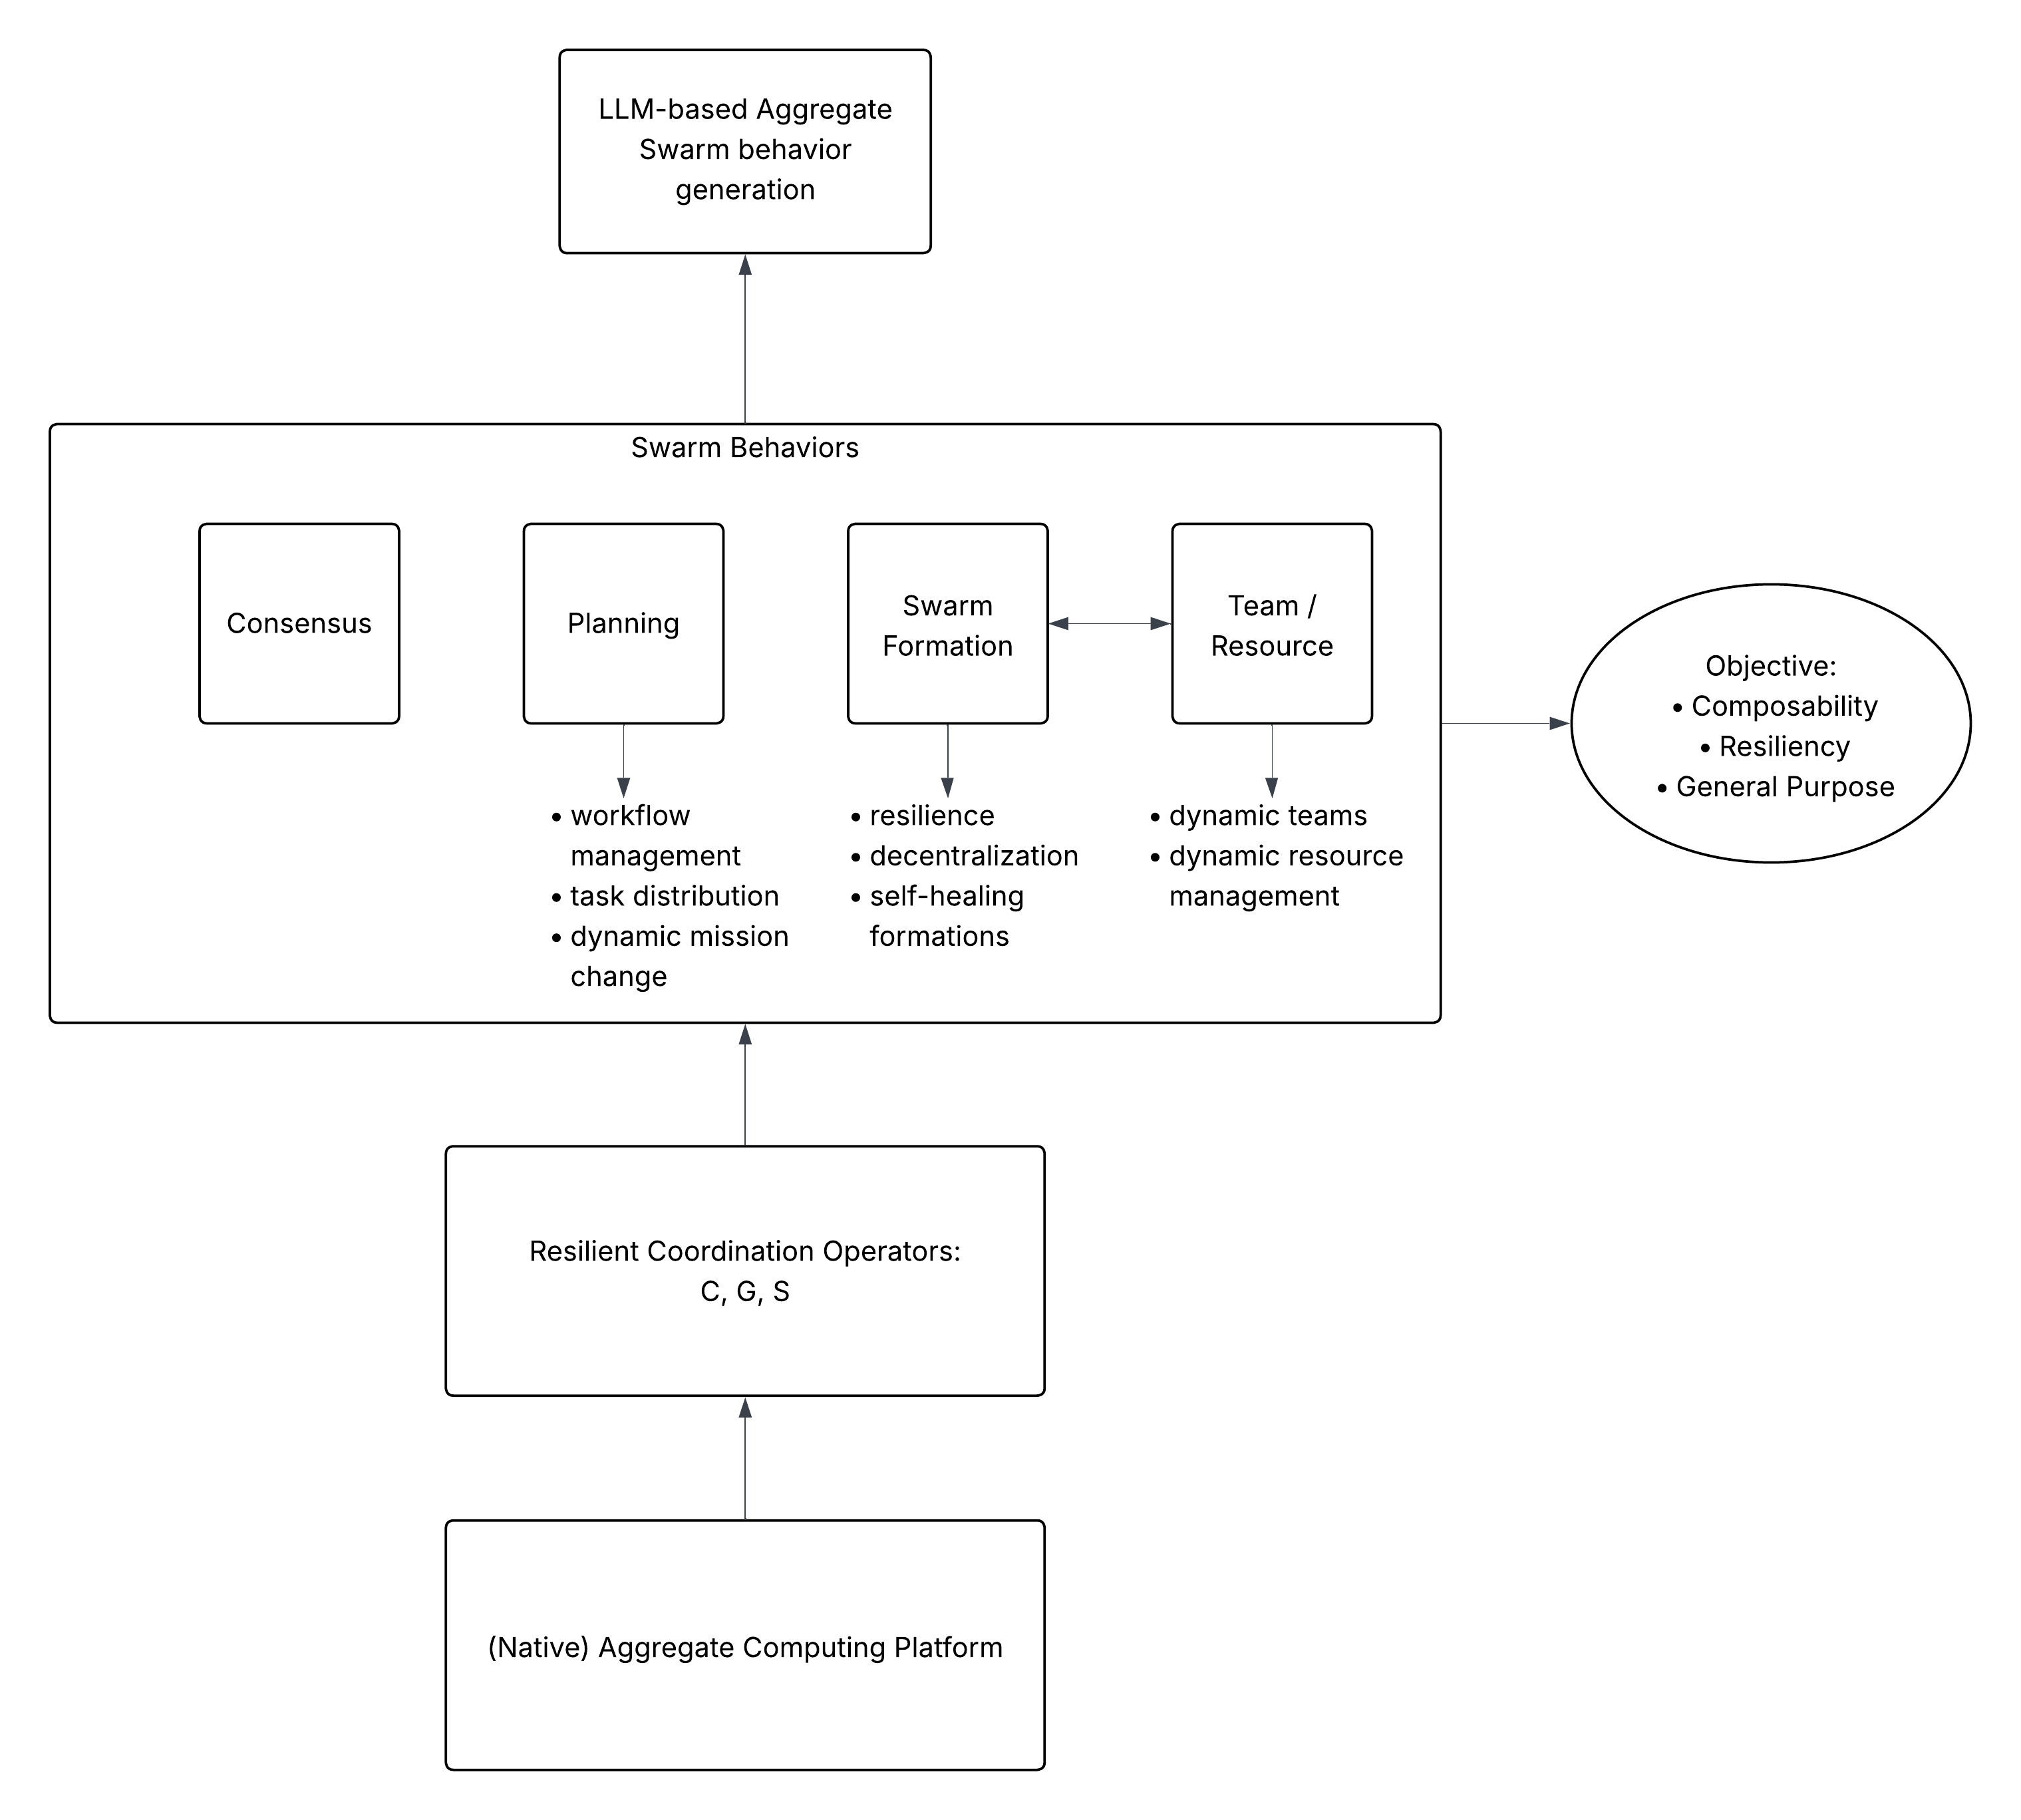
\includegraphics[width=0.7\textwidth]{figures/ResearchProject.png}
	\caption{Overview of the research project}
	 \label{fig:research-project}
\end{figure}

\subsection{Research Goals and Challenges}
\label{sec:challenges}

\subsubsection{Team Management}
Team management refers to the logical subdivision of the swarm resources--e.g., the robots, in order to better tackle a task or collective goal.
Teams may be adaptively derived from local context and could dynamically change based on external, environmental factors or internal factors such as node failure, in spite of
which the collective team configuration should be resilient and self-stabilize in order to converge to the desired goal.

Approaches to team-based collaboration in swarm robotics found in literature vary from evolutionary methods~\cite{ferrante2015evolution} and iterative approaches where complementary
sub-tasks are given to different classes of robots to collaboratively converge to an optimal solution~\cite{ducatelle2010cooperative}. However, there is still a lack of top-down, macro-level
approaches to optimal team management. 

\subsubsection{Swarm Formation}
While teams are a more logic partition of the swarm resources, swarm formation behaviors are a collection of patterns with the aim of adapting the 
spatial, topological structure adopted by the collective. In general, a swarm can have one or more teams and within each team there is a formation.
Recently researched methods for pattern formation in swarm robotics consist of decentralized approaches to flocking formations~\cite{ferrante2012self} and
bio-inspired morphogenetic approaches~\cite{oh2017bio} and low-assumption, bearing-only formation tracking models~\cite{zhao2019bearing} (which lacks actual integration in pratical frameworks). 
However, current implementations are highly case and hardware-specific, and there are currently no proposed methods for top-down collective behaviors that have any guarantee of
timely convergence and resilience to sensor disturbance. 

\subsubsection{Planning}
Planning in swarm robotics is the distributed process by which the collective dynamically coordinates their actions to achieve complex, adaptive objectives.
Given a collective goal, the act of collective planning refers to devising a workflow of tasks that can lead the swarm to achieve said goal, combining behavior, success conditions and task-oriented team management.
Researched approaches found in literature propose a role-based partition of tasks~\cite{sampedro2016flexible}, where robots are given fixed roles within the context of a specific mission, highlighting the lack
of decentralized approaches that let task partitioning and goal pursuing emerge from local interactions.

\subsubsection{Language-based aggregate code generation}
LLM-based code generation already showed promise in various areas of software engineering~\cite{hudson2024software,zhou2025large,he2025llm}. However, if we consider the domain of CAS and swarm robotics in particular, 
a gap remains in language-based program synthesis methods, particularly when LLMs must generate code for specialized domains or languages not well-represented in their training data. This challenge is especially pronounced in niche areas like aggregate computing, where domain-specific constructs and paradigms may be unfamiliar to general-purpose models, potentially limiting the quality and correctness of generated code.
Recent research~\cite{vemprala2024chatgpt} showed the potential of combining LLMs, prompt engineering and, notably, libraries of robot functionalities 
to enact a language-based robot development process. This highlights the potential for developing similar solutions in AC contexts, as the paradigm is by design comprised of simple, functional and composable building blocks that could
be combined by LLM agents to generate aggregate specifications based on constraints gathered with natural language processing.

\subsection{Reference Scenarios}
\label{sec:scenarios}

\paragraph{Disaster Response.} One of the most promising areas is disaster response and search \& rescue. Swarms of inexpensive robots can rapidly explore a disaster site, 
locating survivors or mapping damage much faster than a single robot or human team. 
Aerial drone swarms could coordinate to cover different sectors of a search area, communicate sightings of survivors, and collaboratively haul lightweight relief supplies. 
Their distributed nature means even if some drones crash or lose signal, the rest can complete the mission - a critical advantage in hazardous environments.

\paragraph{Crowd Management/Control.} 
Instead of relying on fixed cameras or isolated sensors, a swarm of aerial and/or ground robots can self-distribute across an event site, ensuring full coverage even as crowds shift.
Using local, sensing-based rules, each robot repels neighbors to avoid clustering and is attracted to lower-density zones, naturally spreading out to fill gaps in sensing coverage
to dynamically track pedestrian densities in public squares, transit hubs, or during mass gatherings.

\paragraph{Digital Twins of Swarms.}
Swarm Digital Twins represent virtual replicas of physical swarm robotic systems, capturing their collective behaviors and interactions in real-time. 
In this scenario, a digital twin of a robot swarm deployed for environmental monitoring continuously integrates real-time sensor data and operational states of each physical robot. 
Leveraging this digital counterpart, operators can anticipate emergent behaviors, optimize swarm performance, and preemptively detect faults or potential disruptions before they manifest in the real system. 
Furthermore, digital twins provide a safe platform for testing and validating new swarm algorithms and coordination strategies prior to physical deployment, significantly reducing experimentation costs and risks. 
By merging real-time physical insights with advanced predictive analytics, swarm digital twins enable more efficient, reliable, and adaptable swarm robotic systems, bridging the gap between theoretical models and practical applications.
% ----------------------------------------
\section{Expected Results}
As a form of result of the proposed project, it is expected to bring \textit{(i)} scientific contributions to CAS engineering, in particular in swarm robotics and collective behavior through AC,
\textit{(ii)} to realize a unified composable API founded on AC to address the open challenges in Section~\ref{sec:challenges}, 
\textit{(iii)} to design a macroprogramming LLM agent capable of translating global specifications into executable local behavior,
\textit{(iv)} validations based on reference scenarios conducted within state of art simulators such as Argos~\footnote{\url{https://www.argos-sim.info/}} and Alchemist~\footnote{\url{https://github.com/AlchemistSimulator/Alchemist}} as well
as in the real-world.

The future vision for the project is to enable the building of complex, resilient and dynamic swarm behaviors through natural languge processing and deploy them in real-world scenarios, some of which could be \textit{(i)} precision agriculture,
\textit{(ii)} environmental monitoring, \textit{(iii)} logistics and warehousing, \textit{(iv)} disaster response and search, 
\textit{(v)} ubiquitous computing with Swarm Digital Twins.

% ----------------------------------------
\section{Lead-time for implementation}
\begin{figure}
	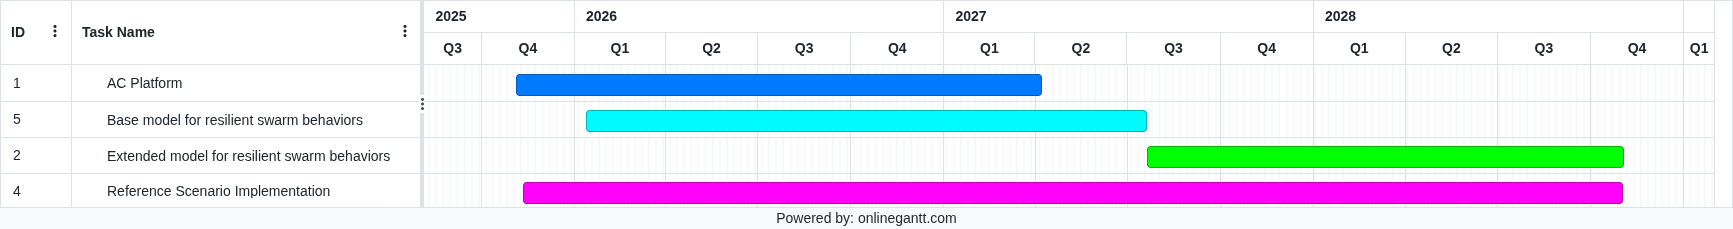
\includegraphics[width=\linewidth]{figures/timeline.png}
	\caption{Hypothetical three year timeline for the project.}
	\label{fig:timeline}
\end{figure}

The Figure~\ref{fig:timeline} shows the hypothetical three-year timeline for the project, subdivided into quarters.

\paragraph{First year.} In the first year will be crucial a deep dive into the research of the state of the art in aggregate computing, FC operators and their properties, as they will lay the foundation of the basic composable building blocks for swarm behavior, such as flocking, pattern formation, consensus and leader election.
Additionally, research in state of the art for LLM-based program synthesis will be foundational to propose an LLM macroprogramming agent, whose development is expected to follow the entire lifecycle of the project, since constructs and concepts will be introduced over time. 
Extensive testing will be conducted firstly by simulating a reference scenario, with the final goal to implement it in the real-world.

\paragraph{Second year.} Within the second year, it is expected to shift focus from the basic building blocks of swarm behavior to the extended library, that will tackle some of the most relevant challenges expressed in Section~\ref{sec:challenges}.
There will also be an increase in prototyping activities, which will first start in a simulated environment.

\paragraph{Third year.} In the third and final year, the focus will predominantly be to finalize the library of resilient swarm behaviors, while also converging to the end of the real-world testbed in the referenced scenario.

% ----------------------------------------
\section{Proposed criteria to be used to assess the findings obtained}

\paragraph{Qualitative.}
The project will be assessed qualitatively by examining the expressiveness, usability, and resilience of the proposed framework in real-world and simulated deployments.  
Key questions include:  
(i) Expressiveness \& composability: possibility to describe a broad spectrum of swarm behaviours concisely. 
(ii) Robustness \& adaptability in the field: how the swarm copes with adversarial events and whether it self‑stabilises to the intended global behaviour.  
(iii) “Democratisation:” Success is achieved if the same aggregate program can run unmodified on heterogeneous hardware classes that include low resource devices.
(iv) Possibility to derive the desired collective behavior from natural language specifications.

\paragraph{Quantitative.}
Experiments need to be rigorously conducted and documented from the beginning of the simulated prototype phase until the end of the reference scenario implementation in the real world.
Detailed quantitative metrics for success need to be expressed while documenting such experiments. 
The metrics gathered will be compared with state-of-the-art swarm robotics frameworks to evaluate performance relative to optimal solutions.
Particular attention will be needed in verifying the correctness of LLM-generated behaviors compared to manually created ones.
As field-testing requires specialized hardware, efforts will be made to secure partnerships for international research stays during the PhD program, facilitating access to necessary equipment for project testing.

\paragraph{Scientific Contributions.}
During the course of the program, it is expected to contribute to the scientific knowledge of CAS engineering and swarm robotics. 
In particular, it is expected to submit papers annually to conferences that are relevant to the field of CAS (such as ACSOS \footnote{\url{https://acsos.github.io/}}) and robotics (such as ICRA \footnote{\url{https://2025.ieee-icra.org/}}),
as well as journals such as TAAS~\footnote{\url{https://dl.acm.org/journal/taas}} and Swarm Intelligence~\footnote{\url{https://www.scimagojr.com/journalsearch.php?q=11700154734&tip=sid}}.
Success will also be evaluated by establishing international collaborations with experts like Prof. Lukas Esterle and Prof. Alessandro Papadopoulos, who have prior collaboration experience with the research group I will work with.
\clearpage

%-----------------------------------------
\renewcommand{\refname}{References}

\bibliographystyle{plain}
\bibliography{latex}

\end{document}
